\documentclass[tikz, preview]{standalone}

\usepackage{amsfonts, amsthm, amssymb, amsmath, stmaryrd, etoolbox}
\usepackage{tikz}
\usepackage[all,2cell]{xy}
\usetikzlibrary{matrix,arrows,shapes,decorations.markings,decorations.pathreplacing}
\definecolor{rewritecolor}{rgb}{0,.9,1}
\tikzset{rewritenode/.style={shape=circle,fill=rewritecolor,scale=0.25,font=\Huge}}
\tikzset{RWopen/.style={shape=circle,draw=black,fill=white,scale=0.5,font=\Huge}}
\tikzset{RWclosed/.style={shape=circle,fill=black,scale=0.5,font=\Huge}}
\tikzset{CDnode/.style={shape=circle,fill=white,scale=.5}}
\tikzset{zxgreen/.style={shape=circle,draw,thick,fill=green}}
\tikzset{zxred/.style={shape=circle,draw,thick,fill=red}}
\tikzset{zxyellow/.style={shape=rectangle,draw,thick,fill=yellow}}
\tikzset{zxdiamond/.style={shape=diamond,fill=black,inner sep=2.75}}
\tikzset{zxopen/.style={shape=circle,draw,thick,inner sep=2pt}}
\tikzset{->-/.style={decoration={markings,mark=at position .5 with {\arrow{>}}},postaction={decorate}}}

\begin{document}
\[
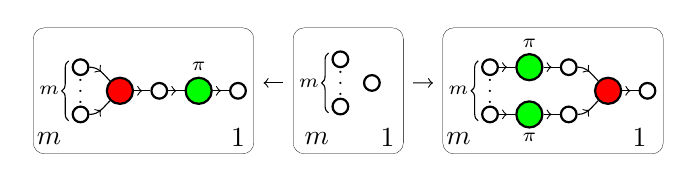
\begin{tikzpicture}
%
%
%
\begin{scope}[shift={(-1,-0.6)}]
\node [zxopen] (v1) at (-0.7,0.4) {};
\node [zxopen] (v2) at (-0.7,-0.2) {};
\node [zxred,label={}] (v3) at (-0.2,0.1) {};
\node [zxgreen,label={[shift={(0,-0.05)}]\scriptsize $\pi$}] (v4) at (0.8,0.1) {};
\node at (-0.7,0.2) {\scriptsize $\vdots$};
\node [zxopen] (v5) at (1.3,0.1) {};
\node [zxopen] (v6) at (0.3,0.1) {};

%
\draw [->-] (v1) to [out=0,in=135] (v3);
\draw [->-] (v2) to [out=0,in=-135] (v3);
\draw [->-] (v3) to (v6);
\draw [->-] (v6) to (v4);
\draw [->-] (v4) to (v5);
%
\node at (-1.1,-0.5) {$m$};
\node at (1.3,-0.5) {$1$};
\node (v11) at (1.5,0.2) {};
\draw [ultra thin, rounded corners] (-1.3,0.9) rectangle (1.5,-0.7);
\draw[decoration={brace,mirror,raise=2pt},decorate]
(v1.north west) -- node [left=2pt] {\scriptsize $m$} (v2.south west); 
\end{scope}
%
%
%
\begin{scope}[shift={(2.7,-0.1)}]
\node [zxopen] (v1) at (-1.1,0) {};
\node [zxopen] (v2) at (-1.1,-0.6) {};
\node [zxopen] (v3) at (-0.7,-0.3) {};
\node (v4) at (-1.1,-0.2) {\scriptsize $\vdots$};

%
\draw [ultra thin, rounded corners] (-1.7,0.4) rectangle (-0.3,-1.2);
\node at (-1.4,-1) {$m$};
\node at (-0.5,-1) {$1$};
\node (v12) at (-1.7,-0.3) {};
\node (v14) at (-0.3,-0.3) {};
\draw[decoration={brace,mirror,raise=2pt},decorate]
(v1.north west) -- node [left=2pt] {\scriptsize $m$} (v2.south west); 
\end{scope}
%
%
%
\begin{scope}[shift={(4.9,-0.5)}]
\node [zxopen] (v1) at (-1.4,0.3) {};
\node [zxopen] (v2) at (-1.4,-0.3) {};
\node [zxgreen,label={[shift={(0,-0.05)}]\scriptsize $\pi$}] (v3) at (-0.9,0.3) {};
\node [zxgreen,label={[shift={(0,-0.65)}]\scriptsize $\pi$}] (v4) at (-0.9,-0.3) {};
\node [zxred] (v5) at (0.1,0) {};
\node [zxopen] (v6) at (0.6,0) {};
\node (v7) at (-1.4,0.1) {\scriptsize $\vdots$};
\node [zxopen] (v8) at (-0.4,0.3) {};
\node [zxopen] (v9) at (-0.4,-0.3) {};

%
\draw [->-] (v1) to (v3);
\draw [->-] (v2) to (v4);
\draw [->-] (v3) to (v8);
\draw [->-] (v8) to [out=0,in=135] (v5);
\draw [->-] (v4) to (v9);
\draw [->-] (v9) to [out=0,in=-135] (v5);
\draw [->-] (v5) to (v6);
%
\node at (-1.8,-0.6) {$m$};
\node at (0.5,-0.6) {$1$};
\draw [ultra thin, rounded corners] (-2,0.8) rectangle (0.8,-0.8);
\node (v13) at (-2,0.1) {};
\draw[decoration={brace,mirror,raise=2pt},decorate]
(v1.north west) -- node [left=2pt] {\scriptsize $m$} (v2.south west);
\end{scope}
%
%
%
\draw [<-] (v11) edge (v12);
\draw [<-] (v13) edge (v14);
\end{tikzpicture}
\]
\end{document}
